\documentclass[letterpaper,11pt]{article}

\usepackage[empty]{fullpage}
\usepackage[x11names]{xcolor}
\usepackage[utf8]{inputenc}
\usepackage[frenchb]{babel}
\usepackage{graphicx}
\usepackage[colorlinks=true, urlcolor=RoyalBlue4, pdftitle={CV Quentin Casasnovas}, pdfauthor={Quentin Casasnovas}, pdfsubject={CV Quentin Casasnovas}]{hyperref}

\raggedbottom
\raggedright
\setlength{\tabcolsep}{0in}

\addtolength{\oddsidemargin}{-0.5in}
\addtolength{\evensidemargin}{-0.5in}
\addtolength{\textwidth}{1.0in}
\addtolength{\topmargin}{-0.5in}
\addtolength{\textheight}{1.0in}

\hypersetup{
  pdfborder=0 0 0}


% Custom commands

\newcommand{\resitem}[1]{\item #1}

\newcommand{\titlecolor}[0]{RoyalBlue4}
\newcommand{\bulletcolor}[0]{darkgray}

\newcommand{\resheading}[1]{
  \vspace{10pt}
  {\Large
        \textsc{\textcolor{\titlecolor}{\textbf{#1}}}
  } \\
  \vspace{-10.5pt}
  \hspace{-1pt}\textcolor{\titlecolor}{\line(1,0){525}}
}

\newcommand{\ressubheading}[4]{
  \vspace{12pt}
  \begin{tabular*}{7.0in}{l@{\extracolsep{\fill}}r}
    \textsc{#1} & #2 \\
    \textsl{#3} & \textit{#4} \\
  \end{tabular*}
  \vspace{4pt}
}

\newcommand{\prettylist}[0]{
  \begin{itemize}
    \renewcommand{\labelitemi}{{\tiny \textcolor{\bulletcolor}{$\bullet$}}}
    \renewcommand{\labelitemiii}{$\cdot$}
}

\newcommand{\projectlist}[0]{
  \begin{tabular}{p{0.03\linewidth}p{0.4\linewidth}p{0.1\linewidth}p{0.4\linewidth}}
    & \begin{itemize}
}

\newcommand{\projectitem}[1]{
  \vspace{3pt}
  \item[ \textcolor{\bulletcolor}{{\tiny $\bullet$}} {\small \textsc{#1}}]
}

\newcommand{\projectsep}[0]{
      \end{itemize} & & \begin{itemize}
}

\newcommand{\projectlistend}[0]{
\end{itemize}
\end{tabular}
}

\newcommand{\acro}[1]{
  \hspace{-1pt}{\small\textsc{#1}}\hspace{-3pt}
}

% Document


\begin{document}

\begin{minipage}{0.40\linewidth}
{\LARGE \textbf{\textcolor{\titlecolor}{Quentin Casasnovas}}}\\
\vspace{2pt}
\begin{tabular}{p{0.007\linewidth}l}
 & {\small \textcolor{\titlecolor}{920 TOEIC}} \\
 & {\small \textcolor{\bulletcolor}{\url{http://uk.linkedin.com/in/quentincasasnovas}}} \\
 & {\small \textcolor{\bulletcolor}{French nationality, 27 years old}} \\
 & {\small \textcolor{\bulletcolor}{quentin@dev-kernel.fr}} \\
 & {\small \textcolor{\bulletcolor}{10 \acro{Av. du Trayas} - \acro{App. C14}}} \\
 & {\small \textcolor{\bulletcolor}{06590 \acro{Theoule sur mer - France}}} \\
 & {\small \textcolor{\bulletcolor}{+33 651 494 310}} \\
\end{tabular}
\end{minipage}
\begin{minipage}{0.54\linewidth}
\begin{flushright}
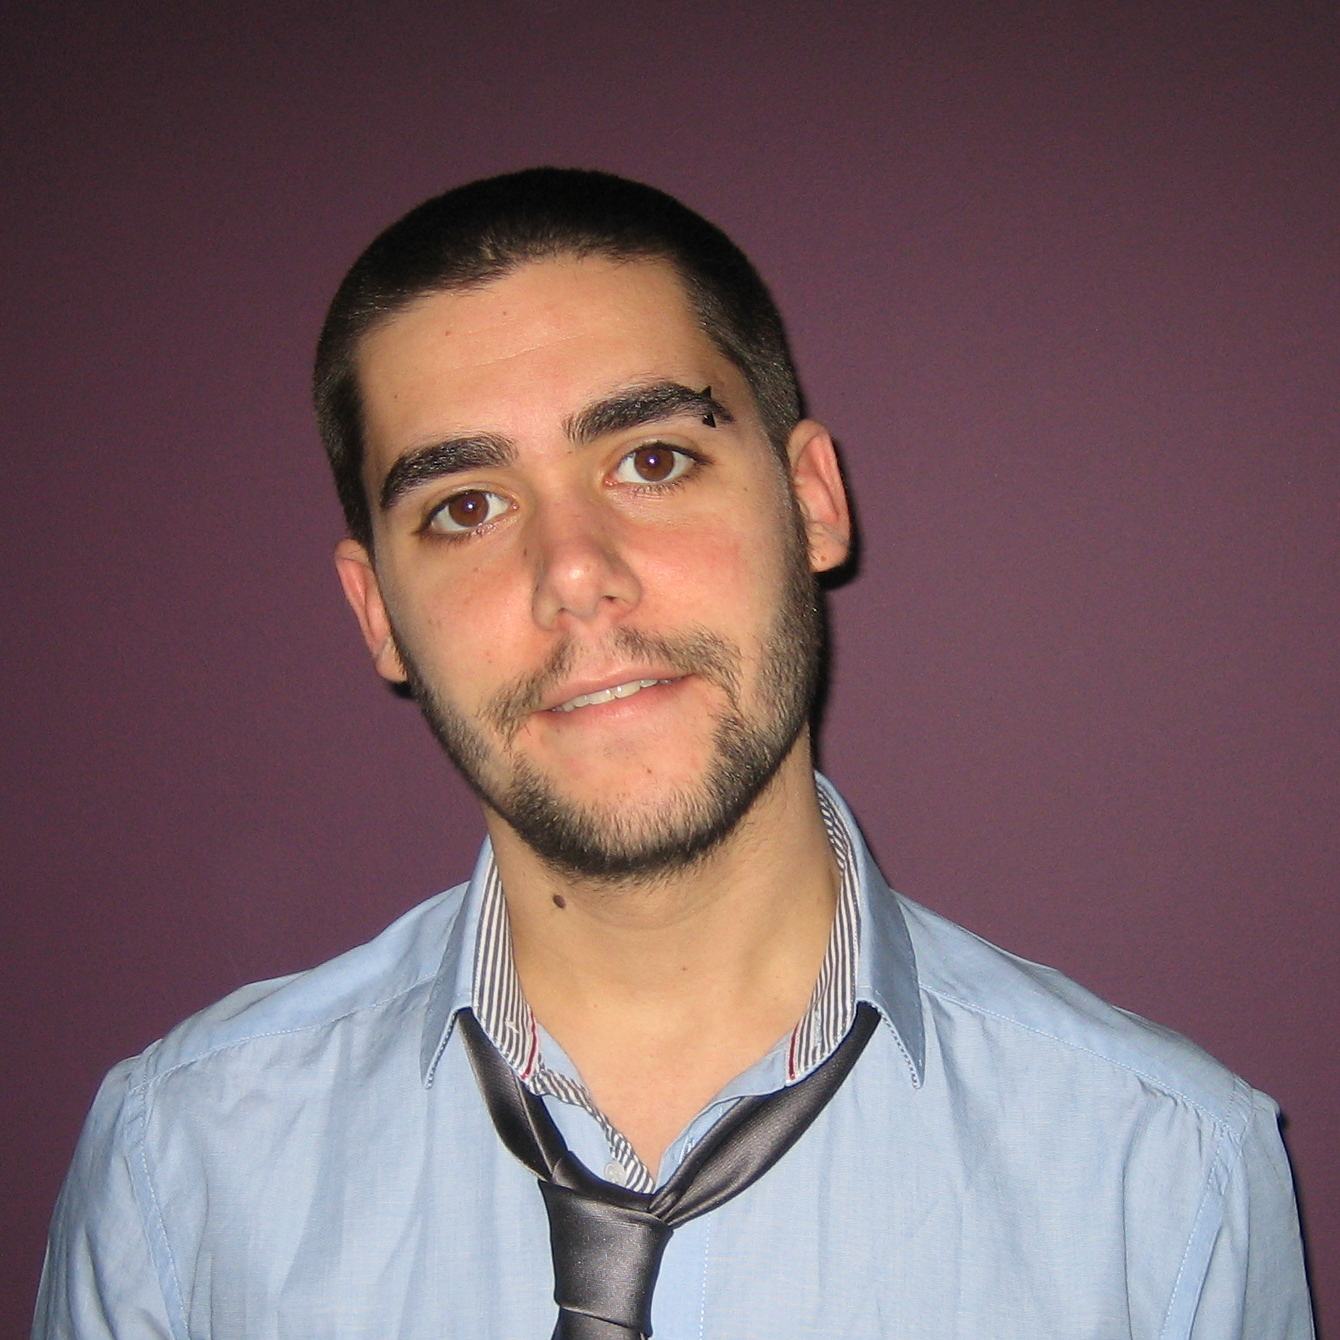
\includegraphics[scale=0.07]{id.png}
\end{flushright}
\end{minipage}

\vspace{8pt}
\resheading{Goals}
\begin{minipage}{0.95\linewidth}
\vspace{10pt}
\paragraph{}
My main area of interest is kernel development, shall it be low level kernel
development such as platform/device driver implementation, or at a higher level
with userland interaction. I'm thrived by challenging projects involving
complex interactions between the hardware all the way through to userland.
\paragraph{}
I'm especially attracted by companies which work with/on open source project
like the Linux kernel, and which have a strong technical/innovation
background. A company putting a lot of effort in R\&D is a plus, so is 
using agile software development methods and valorisating technical
expertise.

\end{minipage}

\vspace{5pt}
\resheading{Experience}
\vspace{3pt}
\prettylist
\item
  \ressubheading{Intel Ultra Mobility Group, Freelance (Dev Kernel Ltd)}{Sophia
    Antipolis, France}{Linux/Android Embedded Engineer}{Sep. 2012 - today}
  \begin{itemize}
    \resitem{Various WiFi/BT chipset bring up on Intel future reference platforms}
    \resitem{Rework Android WiFi stack so it can scale to different WiFi chipset}
    \resitem{Bug fixing (mostly in-kernel) and customer support}
    \resitem{Added ACPI support for SDIO bus in Linux kernel}
  \end{itemize}
\item
  \ressubheading{MathEmbedded, Permanent Contract}{Bristol, England}{ Linux
    Embedded Engineer - Tech Lead}{Dec. 2010 - Sep. 2012}
  \begin{itemize}
    \resitem{Author of a kernel based tracing mechanism to automate \acro{STB}s certification}
    \begin{itemize}
      \resitem{Design/Implementation of the low level plumbing, tech lead}
      \resitem{Requirements capture on site, support and documentation}
    \end{itemize}
    \resitem{Split of grsecurity patch for easier integration on Embedded devices}
    \resitem{Boot time optimizations for different SH4 based HW}
    \resitem{\acro{Linux}/security trainer}
  \end{itemize}
\vspace{1.1pt}\item
  \ressubheading{Scaleo Chip, Final Internship}{Sophia Antipolis,
    France}{Reducing power consumption on \acro{Linux-SMP SoC}}{Feb. 2010 -
    Sep. 2010}
  \begin{itemize}
    \resitem{Implementation of cpu hotplug/hotunplug for sparc architecture for \acro{Linux}} 
    \resitem{Dynamically stop/start back CPU depending on system load}
    \resitem{Development of Python/Qt UI to monitor the current consumption of the platform through USB}
  \end{itemize}
\vspace{1.1pt}\item
  \ressubheading{DCNS, Internship}{Toulon, France}{Improvement of the HMI of a sub-marine simulator}{Jun. 2008 - Aug. 2008}
  \begin{itemize}
    \resitem Development in\acro{OpenMotif/C}
  \end{itemize}
\item
  \ressubheading{McDonald's Grand Ciel, Permanent contract}{La Garde,
    France}{Teammate then team leader}{Sep. 2004 - Apr. 2008}
  \begin{itemize}
    \resitem Manager responsible for training and supplies the last two years
  \end{itemize}
\end{itemize}

\clearpage

\resheading{Education}
\prettylist
\item
  \ressubheading{EPITA}{Paris XIII, Île de France}{Engineering degree -
    Embedded and Real Time systems}{Sep. 2008 - Sep. 2010}
  \begin{itemize}
    \resitem{Member of the research laboratory \href{https://www.lse.epita.fr}{\acro{LSE}} (Laboratoire Systèmes
      d'Exploitation)}
  \end{itemize}
\item \ressubheading{USTV}{La Garde, Var}{Master 1 in Systems Informationnal
    Security}{Sep. 2004 - Apr. 2008}
  \begin{itemize}
    \resitem{Tutoring of 1\textsuperscript{st} year students}
  \end{itemize}
\item
  \ressubheading{High School Jean Aicard}{Hyères, Var}{Scientific High School
    Graduation - Math option}{Sep. 2001 - Jul. 2004}
  \begin{itemize}
    \resitem{One semester in Toronto, Canada}
  \end{itemize}
\end{itemize}

\resheading{Skills}
\begin{description}
\item[Operating systems]
  Strong\acro{GNU/Linux; Android}
\item[Languages]
  \acro{Expert in C; Already worked with C++, D, Python, Perl, Shell, Ada}
\item[Things I use every day]
  \acro{git, emacs, ssh, bitlbee, gcc, gentoo, latex, gdb, toothbrush}
\end{description}
\vspace{-14pt}

\begin{tabular}{p{0.47\linewidth}p{0.05\linewidth}p{0.38\linewidth}}
\begin{description}
\item[Miscellaneous]
  {\small
    \begin{itemize}
    \item[ ]
    \item Fluent english speacker
    \item Good problem solving skills
    \item Deliver secure, well documented code
    \end{itemize}
  }
\end{description}
 & &
\begin{description}
\item[Human]
  {\small
    \begin{itemize}
    \item[ ]
    \item Good communication skills
    \item Excellent adaptability
    \item Strong team spirit
    \end{itemize}
  }
\end{description}
\end{tabular}

\resheading{Misc}
\begin{description}
\item Driver licence and coastal licence. I like fishing, reading and I love barbecues :) 
\item I swim regularly and play squash at least 2 times per week.
\end{description}

\end{document}
